\section{栈和队列}
\begin{frame}[fragile]
  \frametitle{栈和队列}
  ~
\end{frame}

\subsection{基本概念}
\begin{frame}[fragile]
  \frametitle{栈和队列:两种特殊的线性表}
  \begin{columns}
    \begin{column}[T]{0.5\linewidth}
      \begin{tcolorbox}[colframe=red!80, height=6.5cm, title=栈/Stack]
        \small
        \begin{itemize}
        \item 限制仅在表的一端进行插入和删除。
        \item 通常称插入、删除的一端为栈顶 (Top),另一端为栈底 (Bottom)
        \item LIFO:Last In First Out
        \end{itemize}
      \end{tcolorbox}
    \end{column}
    \begin{column}[T]{0.5\linewidth}
      \begin{tcolorbox}[colframe=blue!80, height=6.5cm, title=队/Queue]
        \small
        \begin{itemize}
        \item 限制仅在表的一端进行插入、在另一端进行删除。
        \item 允许插入的一端称队尾 (rear),允许删除的一段称为队头 (front)。
        \item FIFO:First In First Out
        \end{itemize}
      \end{tcolorbox}
    \end{column}
  \end{columns}
\end{frame}

\begin{frame}[fragile]
  %\frametitle{不同场合下的栈}
  \begin{center}
    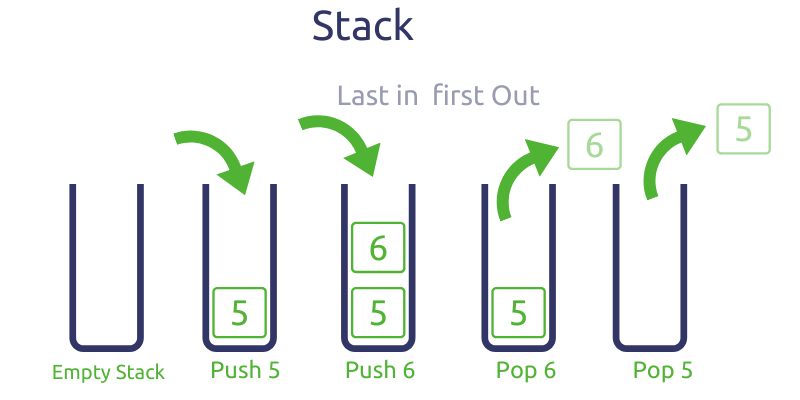
\includegraphics[width=0.7\textwidth]{figs/stack/Stack-data-structure.png}
  \end{center}

  \begin{easylist}
    & 操作系统中的栈

    && 由编译器自动分配释放 ,存放函数的参数值,局部变量的值等。栈使用的是一级缓
    存,被调用时处于存储空间中,调用完毕立即释放。

    & 数据结构中的栈

    && 一种后进先出的数据结构
  \end{easylist}
\end{frame}

\begin{frame}[fragile]
  \frametitle{为什么设计栈、研究栈?}
  \scriptsize
  \begin{itemize}
  \item 栈的一个重要应用是在程序设计中实现递归,从而使许多实际问题大大简化。
  \end{itemize}

  \begin{columns}
    \begin{column}[T]{0.5\linewidth}
      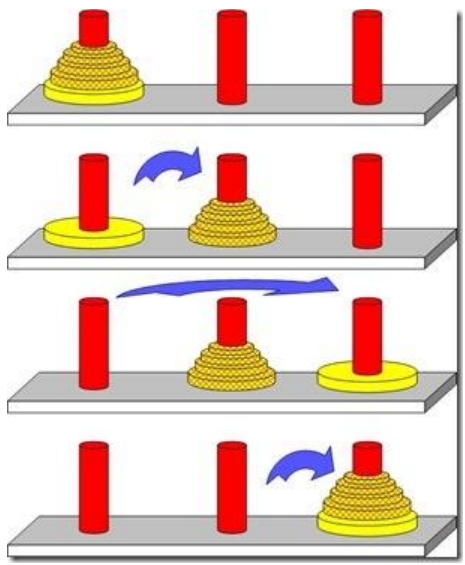
\includegraphics[width=0.9\textwidth]{figs/stack/Tower-Of-Hanoi-1.png}
    \end{column}
    \begin{column}[T]{0.5\linewidth}
        \begin{itemize}
        \item 上帝创造世界的时候做了三根金刚石柱子,在一根柱子上从下往上按大小顺
          序摞着64片黄金圆盘。上帝命令婆罗门把圆盘从下面开始按大小顺序重新摆放在
          另一根柱子上,并且规定一次只能移动一个圆盘,在小圆盘上不能放大圆盘。
        \item 有预言说,这件事完成时宇宙会在一瞬间闪电式毁灭。也有人相信婆罗门至
          今还在一刻不停地搬动着圆盘。
        \item \color{red} 18,446,744,073,709,551,615次搬动才能挪完64片金盘!
        \end{itemize}
    \end{column}
  \end{columns}
\end{frame}

\begin{frame}[fragile]
  \frametitle{举例:计算n的阶乘}
  \scriptsize
  \begin{columns}
    \begin{column}[T]{0.4\linewidth}
      \begin{minted}{java}
        int factorial (int n) {
          int  f ;
          if (n==1) f=1;
          else f=n*fact (n-1) ;
          return f;
        }
      \end{minted}
    \end{column}
    \begin{column}[T]{0.6\linewidth}
      \begin{enumerate}
      \item 将调用函数的现场(各寄存器的值,中断时的程序地址等)入栈,转入被调函数;
      \item 执行被调函数,如又调用其它函数,则执行上述步骤;
      \item 被调函数执行完,取栈顶的值,恢复调用函数时的现场,根据现场中的指令地
        址,恢复调用函数在中断处继续执行。
      \end{enumerate}
    \end{column}
  \end{columns}
  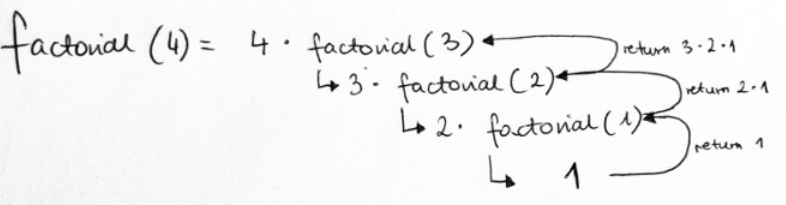
\includegraphics[width=0.9\textwidth]{figs/stack/factorial.png}
\end{frame}

\subsection{栈的存储表示方法}
\begin{frame}[fragile]
  \frametitle{栈的存储表示方法}
  \begin{tcolorbox}[colframe=red]
    请考虑其常用操作。试想选用顺序存储还是链式存储?
  \end{tcolorbox}

  \begin{columns}
    \begin{column}[T]{0.1\textwidth}
      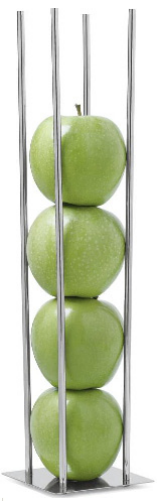
\includegraphics[width=1cm]{figs/stack/apple.png}
    \end{column}
    \begin{column}[T]{0.5\textwidth}
      \begin{easylist}
        & 特点:后进先出

        && 1、经常性的在栈顶插入新元素,以及取栈顶元素;

        && 2、无须访问非栈顶元素。
      \end{easylist}
    \end{column}
    \begin{column}[T]{0.4\textwidth}
      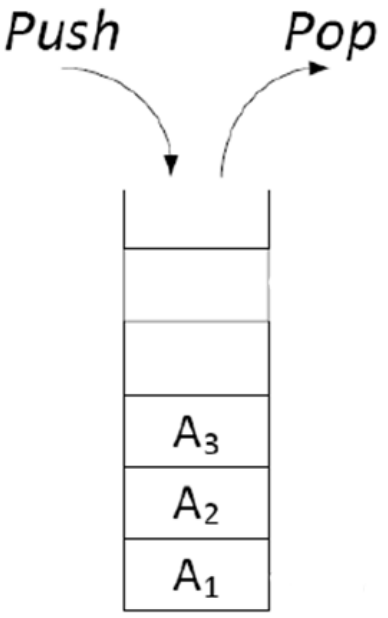
\includegraphics[width=3cm]{figs/stack/pushpop.png}
    \end{column}
  \end{columns}
\end{frame}

\begin{frame}[fragile]
  \frametitle{1. 顺序栈}
  \begin{columns}
    \begin{column}[T]{0.5\linewidth}
      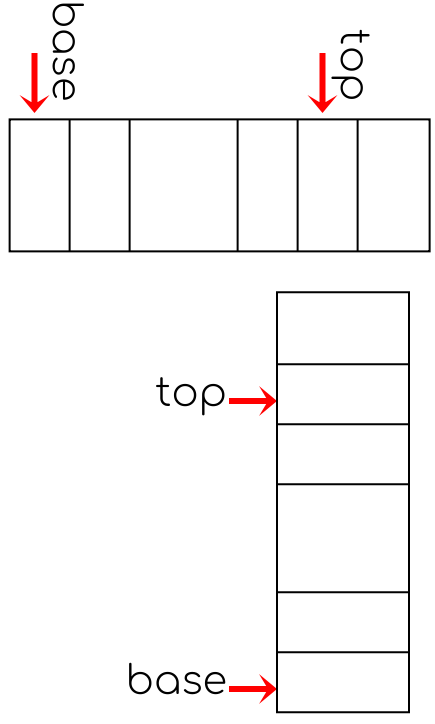
\includegraphics[width=0.7\textwidth]{figs/stack/seq-stack.png}
    \end{column}
    \begin{column}[T]{0.5\linewidth}
      \begin{enumerate}
      \item 顺序栈中元素用地址连续的存储单元依次存放;
      \item 栈底位置固定不变;
      \item 栈顶位置top随着进栈和出栈的操作而变化。
      \end{enumerate}

      顺序栈类型定义:

      \begin{minted}{c}
        class stack<Elem>{
          Object[] data;
          int top;
          int maxSize;
        } SeqStack;
      \end{minted}
    \end{column}
  \end{columns}
\end{frame}

\begin{frame}[fragile]
  \begin{easylist}
    & 动态分配
    && 先为栈分配一个初始容量,在栈的空间不够使用时再逐段扩大。

    & 指针base
    && 始终指向栈底位置,如果base为NULL表示栈不存在;

    & 指针top
    && 初值指向栈底,即top = =base,表示栈空;(不唯一)
    && 每当插入新的栈顶元素,指针top++;
    && 每当删除栈顶元素,指针top--;
    && 非空栈中的栈顶指针始终在栈顶元素的下一个位置上。
  \end{easylist}

  \centering
  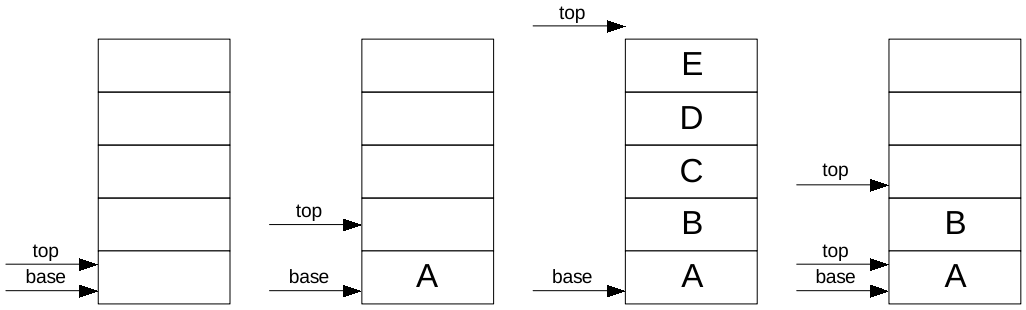
\includegraphics[width=0.8\textwidth]{figs/stack/stack-demo.png}
\end{frame}

\begin{frame}[fragile]
  \begin{columns}
    \begin{column}[T]{0.5\linewidth}
      \begin{tcolorbox}[height=8cm]
        对于顺序栈,入栈需要判栈是否满,是则需要中止、或重新分配空间,否则出现空间溢出。

        \begin{minted}{java}
public Boolean push (Elem e) {
  if ( top==maxSize) {
    print("栈已满");
    return false;
  }
  data[top++] = e;
  return true;
}
        \end{minted}
      \end{tcolorbox}
    \end{column}
    \begin{column}[T]{0.5\linewidth}
      \pause
      \begin{tcolorbox}[height=8cm]
        出栈首先要判断栈是否为空;否则栈空时进行操作将出现下溢错误。

        \begin{minted}{java}
public Elem pop() {
  if(top==base) {
    return null;
  } else {
    top = top-1
    return data[top];
  }
}
        \end{minted}
      \end{tcolorbox}
    \end{column}
  \end{columns}
\end{frame}


\subsection{链栈}
\begin{frame}[fragile]
  \frametitle{2. 链栈}

  \small

  \begin{columns}
    \begin{column}[T]{0.7\linewidth}
      \begin{easylist}
        & 链栈有无栈满溢出问题?

        & 指针如何指?

        && 从栈顶依次向后指,因为操作主要是在栈顶插入、删除,经常需要根据栈顶元
        素找次顶元素。

        & 是否要加头结点?

        && No. 因为头部插入不会出现处理不一致的问题.
      \end{easylist}

      写出链栈的类型定义:

      \begin{minted}{java}
        class Node{
          Elem data;
          Node next;
        }

        Node  top ; // 链栈
      \end{minted}
    \end{column}
    \begin{column}[T]{0.3\linewidth}
      \scalebox{0.8}{
        \begin{tikzpicture}[fill=red, box/.style={draw, minimum width=0.85cm, minimum height=0.8cm, fill=red!5}]
	        \draw node[] (base) {$base$}
          node[box, thick, right=of base] (d1) { 9 }   node[box, right=0 of d1] (p1) {}
          node[box, above=of d1] (d2) {45}  node[box, right=0 of d2] (p2) {}
          node[box, above=of d2] (d3) {25}  node[box, right=0 of d3] (p3) {$\wedge$}
	        node[left= of d3] (top) {$top$};

          \path (base) edge[draw, dashed, thick, ->] (d1) (top) edge[draw=red, thick, ->] (d3);
		      \path (p1.center) edge[draw=red,  thick, ->, out=45, in=200] (d2) (p2.center) edge[draw=red, thick, in=200, ->] (d3);
        \end{tikzpicture}
      }
    \end{column}
  \end{columns}
\end{frame}

\begin{frame}[fragile]
% \frametitle{链栈基本操作}

  请尝试写出入栈出栈的算法

  \begin{minted}{java}
    public push (Elem e) {
      //是否还要判断栈是否满?
      top=new Node(e, top);
      return OK;
   }

   public pop( ){
     //是否还要判断栈是否空?
     e=top;
     top=top.next;
     e.next=null;
     return e.data;
}
  \end{minted}

\end{frame}

\begin{frame}[fragile]
  \frametitle{栈的应用}
  迷宫求解(见PPT)
\end{frame}

\section{队列}

\begin{frame}[fragile]
  \frametitle{队/Queue}
   \begin{columns}
    \begin{column}[T]{0.5\linewidth}
      \begin{tcolorbox}[colframe=blue!80, height=6.5cm, title=队/Queue]
        \small
        \begin{itemize}
        \item 限制仅在表的一端进行插入、在另一端进行删除。
        \item 允许插入的一端称队尾 (rear),允许删除的一段称为队头 (front)。
        \item FIFO:First In First Out
        \end{itemize}
      \end{tcolorbox}
    \end{column}
    \begin{column}[T]{0.5\linewidth}
      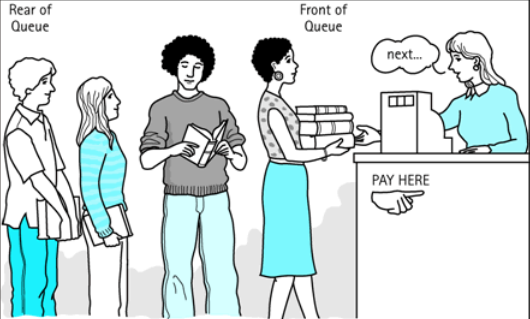
\includegraphics[width=0.9\textwidth]{figs/queue/queueofpeople.png}

      \begin{itemize}
      \item 比如生活中排队购物、操作系统中的作业排队等。
      \end{itemize}
    \end{column}
  \end{columns}
\end{frame}


\subsection{队的存储表示方法}
\begin{frame}[fragile]
  \frametitle{队的存储表示方法}

  \begin{itemize}
  \item 队也有两种存储表示方法:顺序队、链队
  \item 顺序队:利用地址连续的存储单元依次存放数据元素。
  \end{itemize}

  \begin{columns}
    \begin{column}[T]{0.5\linewidth}
      \scalebox{0.7}{
        \begin{tikzpicture}[scale=0.5, box/.style={draw, minimum width=1.2cm, minimum height=0.7cm}]
		      \draw node[box] (a0) {A}
	        node[box, right=0 of a0] (a1) {B}
	        node[box, right=0 of a1] (a2) {C}
	        node[box, right=0 of a2] (a3) {}
          node[box, right=0 of a3, minimum width=2cm] (amore) {$\cdots$}
	        node[box, right=0 of amore] (alast) {}
		      node[above=0 of a0] {0}
				  node[above=0 of a1] {1}
				  node[above=0 of a2] {2}
				  node[above=0 of a3] {3}
				  node[above=0 of amore] {$\cdots$}
				  node[above=0 of alast] {$MaxLen-1$}
	        node[below=0.7cm of a0] (front) {$front$}
	        node[below=0.7cm of a2] (rear) {$rear$};

			    \draw[draw=red, thick, -Latex] (front) -> (a0);
          \draw[draw=red, thick, -Latex] (rear) -> (a2);
        \end{tikzpicture}
      }
    \end{column}
    \begin{column}[T]{0.5\linewidth}
      请写出顺序队的类型定义:

      \begin{minted}{java}
        class SeqQueue{
          ElemType  data[ ];
          int maxsize;
          int rear; //队尾,以此计算队长
        } // 可否??
      \end{minted}
    \end{column}
  \end{columns}
\end{frame}
